\documentclass[11pt,a4paper]{article}

% ------------------------------------------------------------------
% Packages
% ------------------------------------------------------------------
\usepackage[utf8]{inputenc}
\usepackage[T1]{fontenc}
\usepackage[english]{babel}
\usepackage[margin=2.5cm]{geometry}
\usepackage{amsmath}
\usepackage{booktabs}
\usepackage[htt]{hyphenat}
\usepackage{tabularx}
\usepackage{float}
\usepackage{enumitem}
\usepackage{xcolor}
\usepackage{listings}
\usepackage{tikz}
\usetikzlibrary{shapes.geometric, arrows.meta, positioning}
\usepackage{hyperref}

\setlength{\emergencystretch}{3em}
\hypersetup{colorlinks=true, linkcolor=blue!60!black, urlcolor=blue!60!black}

% ------------------------------------------------------------------
% JSON style
% ------------------------------------------------------------------
\definecolor{jsonstr}{RGB}{163,21,21}
\definecolor{jsonbg}{RGB}{247,247,247}

\lstdefinelanguage{json}{
  basicstyle=\ttfamily\small,
  showstringspaces=false,
  columns=fullflexible,
  keepspaces=true,
  upquote=true,
  breaklines=true,
  frame=single,
  rulecolor=\color{gray!40},
  backgroundcolor=\color{jsonbg},
  stringstyle=\color{jsonstr},
  string=[s]{"}{"},
  comment=[l]{//},
  commentstyle=\color{gray}\itshape,
  literate={á}{{\'a}}1 {é}{{\'e}}1 {í}{{\'i}}1 {ó}{{\'o}}1 {ú}{{\'u}}1 {ñ}{{\~n}}1
}
\lstset{language=json}

\newcommand{\apiep}[2]{\texttt{\textbf{#1}~#2}}

% ------------------------------------------------------------------
\title{\textbf{Pricing Engine Module}\\[4pt]\large Architecture, Data Architecture and Decision Record}
\author{}
\date{}

\begin{document}
\maketitle
\tableofcontents
\newpage

% ==================================================================
\section{Service Architecture}
% ==================================================================

\subsection{Definition}
The Pricing Engine is a microservice responsible for \textbf{calculating,
managing, versioning and publishing} the price of every accommodation on the
platform. The price of an accommodation is expressed as
\[
  \text{FinalPrice} = \text{BasePrice} \times \text{Multiplier}
\]
where the \emph{base price} is set by the host and the \emph{multiplier} is
produced by the service from three groups of indicators:

\begin{enumerate}[label=\textbf{\arabic*.}]
  \item \textbf{Demand indicators} (source: Search Engine and bookings, per zone):
  \begin{itemize}
    \item \emph{Unique searches} for a zone within a date range.
    \item \emph{Search-to-booking conversion rate}:
      \[
        \text{Conversion} = \frac{\text{ConfirmedBookings}}{\text{UniqueSearches}} \times 100
      \]
    \item \emph{Occupancy rate}, measured in nights, because an accommodation
      may be occupied only for part of an interval:
      \[
        \text{Occupancy} = \frac{\text{BookedNights}}{\text{TotalAvailableNights}} \times 100
      \]
  \end{itemize}
  \item \textbf{Contextual indicators} (source: Google Events API through SerpAPI):
  events near the zone, with their address, date range and estimated attendance.
  \item \textbf{Host configuration} (source: Accommodation Management):
  base price (fixed by the host, or suggested by the engine), price limits
  (minimum and maximum), and particular rules such as cleaning fee, maximum
  capacity and extra-guest fee.
\end{enumerate}

Zones are the geographic areas defined by the Maps module; every indicator
and every batch is computed per zone.

\paragraph{Multiplier tiers.}
The decision engine is a classical (supervised) machine-learning
\emph{classifier}. It does not output a free continuous value; it selects one
of three discrete tiers, which keeps prices explainable and bounded:

\begin{table}[H]
  \centering
  \begin{tabular}{@{}cll@{}}
    \toprule
    \textbf{Multiplier} & \textbf{Tier} & \textbf{Meaning} \\
    \midrule
    1.02 & Low    & Minimum platform margin (2\,\%); applied by default \\
    1.07 & Medium & Moderate demand and/or relevant events \\
    1.15 & High   & Maximum platform margin (15\,\%) \\
    \bottomrule
  \end{tabular}
  \caption{Discrete multiplier tiers.}
\end{table}

\paragraph{Guardrails.} After the tier is chosen, the final price is clamped
to the host limits:
\[
  \text{FinalPrice} = \min\bigl(\max(\text{BasePrice}\times m,\ \text{MinPrice}),\ \text{MaxPrice}\bigr)
\]
To guarantee the 2\,\% minimum margin, a host configuration is only accepted
if $\text{MaxPrice} \geq 1.02 \times \text{BasePrice}$ and
$\text{MinPrice} \leq \text{BasePrice}$ (otherwise \texttt{400}). If the
model is unavailable or an indicator is missing, the service falls back to
the \textbf{1.02} tier and marks the version as \texttt{fallback}.

\subsection{Architectural style and triggers}
The service follows an \textbf{event-driven} architecture. It consumes and
publishes events through a message broker and processes work
\textbf{asynchronously and in batches}, scaling horizontally (one worker per
zone batch partition).

\begin{table}[H]
  \centering
  \begin{tabularx}{\textwidth}{@{}lXl@{}}
    \toprule
    \textbf{Event} & \textbf{Origin and effect} & \textbf{Scope} \\
    \midrule
    \texttt{ZonePricingBatchRequested} & Emitted by a scheduler on the
      1st day of every month (00:00, America/Bogota), one event per zone.
      Recalculates every active accommodation in the zone for that month. & Zone (batch) \\
    \texttt{AccommodationCreated} & Emitted by Accommodation Management.
      Calculates the first price using the current month's zone snapshot. & Single \\
    \texttt{HostConfigUpdated} & Emitted by Accommodation Management (or
      received via \texttt{POST /pricing/update}). Recalculates the current
      month's price with the new configuration. & Single \\
    \texttt{PriceMultiplierPublished} & \textbf{Published} by the Pricing
      Engine after each new version; consumed by Accommodation Management. & Output \\
    \bottomrule
  \end{tabularx}
  \caption{Events handled and published by the service.}
\end{table}

\subsection{API access}

\subsubsection{Exposed endpoints}
\begin{description}[style=nextline]
  \item[\apiep{POST}{/pricing/quote}]
  Calculates the multiplier for a single accommodation (used for new
  accommodations and manual recalculations). It calls the indicator
  components and Accommodation Management internally.\\
  Body: \texttt{accommodationId}, \texttt{zoneId}, \texttt{period}
  (\texttt{YYYY-MM}).\\
  Codes: \texttt{201} created, \texttt{400} invalid body, \texttt{404}
  accommodation or zone not found, \texttt{500} internal error.
  \item[\apiep{POST}{/pricing/update}]
  Receives a changed host configuration (base price, limits, rules),
  validates the guardrails and enqueues a recalculation.\\
  Codes: \texttt{202} accepted, \texttt{400} invalid configuration,
  \texttt{404} not found, \texttt{500}.
  \item[\apiep{POST}{/pricing/batches}]
  Internal (scheduler or operators). Enqueues a monthly batch for one zone.
  Idempotent on \texttt{(zoneId, period)}.\\
  Codes: \texttt{202} accepted, \texttt{409} batch already exists,
  \texttt{400}, \texttt{500}.
  \item[\apiep{GET}{/pricing/\{accommodationId\}/current}]
  Returns the price version in force. Codes: \texttt{200}, \texttt{404}, \texttt{500}.
  \item[\apiep{GET}{/pricing/\{accommodationId\}/history}]
  Returns the versioned price history (query: \texttt{from}, \texttt{to},
  \texttt{limit}). Codes: \texttt{200}, \texttt{404}, \texttt{500}.
\end{description}

\subsubsection{Internal indicator endpoints}
\begin{description}[style=nextline]
  \item[\apiep{GET}{/demand?zoneId=\&period=}]
  Returns the demand snapshot of a zone for the previous (closed) month.
  Codes: \texttt{200}, \texttt{400}, \texttt{404} no snapshot, \texttt{500}.
  \item[\apiep{GET}{/events?zoneId=\&from=\&to=}]
  Returns the events in a zone for a date range.
  Codes: \texttt{200}, \texttt{400}, \texttt{500}.
\end{description}

\subsection{Data owned by the service}
The Pricing Engine is the single source of truth for:
\begin{itemize}
  \item \textbf{Price versions}: every calculated multiplier and final price,
    append-only, with the indicator snapshot that produced it.
  \item \textbf{Batch runs}: status of each monthly zone batch.
  \item \textbf{Zone demand snapshots}: monthly aggregates derived from the
    Search Engine and bookings.
  \item \textbf{Zone events}: normalized events obtained from SerpAPI.
\end{itemize}
Host configuration is \emph{not} owned by this service; it belongs to
Accommodation Management and is only read. The structure of each owned
entity is shown in Section~\ref{sec:data}.

\subsection{Processing pipeline}
\begin{enumerate}
  \item \textbf{Snapshot closing (last day of month, 23:00).} DemandIndicators
    aggregates the month's unique searches, confirmed bookings and
    booked/available nights per zone from the Search Engine and stores the
    snapshot. ContextIndicators fetches next month's events per zone from
    SerpAPI and stores them.
  \item \textbf{Trigger (1st day of month, 00:00).} The scheduler emits one
    \texttt{ZonePricingBatchRequested} per zone.
  \item \textbf{Collection.} The worker loads the zone demand snapshot
    (\texttt{GET /demand}), the zone events for the month
    (\texttt{GET /events}) and the host configuration of every active
    accommodation in the zone (Accommodation Management, paginated).
  \item \textbf{Decision.} A feature vector is built per accommodation and
    the ML classifier selects a tier (1.02, 1.07 or 1.15).
  \item \textbf{Guardrails.} The final price is computed and clamped to the
    host limits; missing data leads to the 1.02 fallback.
  \item \textbf{Versioning.} A new price version is written to the price
    history store (idempotency key: \texttt{accommodationId + period + trigger + hostConfigVersion}).
  \item \textbf{Publication.} A \texttt{PriceMultiplierPublished} event is
    emitted; Accommodation Management applies the new price.
\end{enumerate}
Single-accommodation events (\texttt{AccommodationCreated},
\texttt{HostConfigUpdated}) run steps 3--7 for one accommodation using the
already closed zone snapshot.

\subsection{Component diagram}
\begin{figure}[H]
\centering
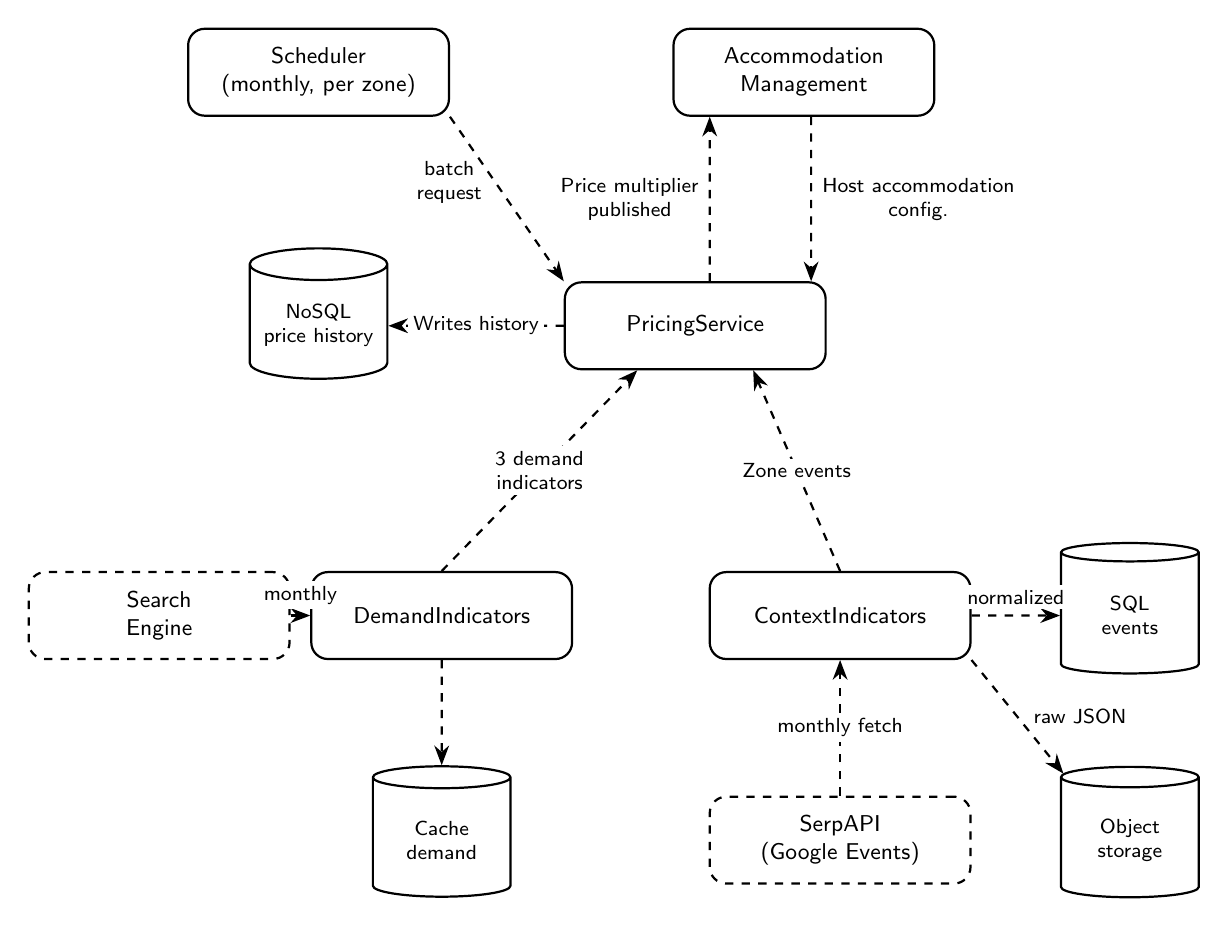
\begin{tikzpicture}[
  scale=0.92, transform shape,
  font=\sffamily\small,
  >={Stealth[length=2.5mm]},
  svc/.style={draw, thick, rounded corners=6pt, minimum width=3.6cm,
              minimum height=1.2cm, align=center, fill=white},
  ext/.style={svc, dashed},
  db/.style={cylinder, shape border rotate=90, draw, thick, aspect=0.25,
             minimum width=1.9cm, minimum height=1.8cm, align=center, fill=white,
             font=\sffamily\footnotesize},
  flow/.style={->, dashed, thick},
  lbl/.style={fill=white, inner sep=2pt, align=center, font=\sffamily\footnotesize}
]
  \node[svc] (sched)   at (-5.2, 5)   {Scheduler\\(monthly, per zone)};
  \node[svc] (acc)     at (1.5, 5)      {Accommodation\\Management};
  \node[svc] (pricing) at (0, 1.5)    {PricingService};
  \node[db]  (nosql)   at (-5.2, 1.5) {NoSQL\\price history};
  \node[svc] (demand)  at (-3.5,-2.5) {DemandIndicators};
  \node[svc] (context) at (2,-2.5)    {ContextIndicators};
  \node[db]  (sql)     at (6,-2.5)    {SQL\\events};
  \node[db]  (cache)   at (-3.5,-5.6) {Cache\\demand};
  \node[db]  (obj)     at (6,-5.6)    {Object\\storage};
  \node[ext] (search)  at (-7.4,-2.5) {Search\\Engine};
  \node[ext] (serp)    at (2,-5.6)    {SerpAPI\\(Google Events)};

  \draw[flow] (sched.south east) -- node[lbl, pos=0.4, left=3pt, fill=none]{batch\\request} (pricing.north west);
  \draw[flow] ([xshift=0.2cm]pricing.north) -- node[lbl, left=2pt, fill=none]{Price multiplier\\published}
              ([xshift=-1.3cm]acc.south);
  \draw[flow] ([xshift=0.1cm]acc.south) -- node[lbl, right=2pt, fill=none]{Host accommodation\\config.}
              ([xshift=1.6cm]pricing.north);
  \draw[flow] (pricing.west) -- node[lbl]{Writes history} (nosql.east);
  \draw[flow] (demand.north) -- node[lbl]{3 demand\\indicators} ([xshift=-0.8cm]pricing.south);
  \draw[flow] (context.north) -- node[lbl]{Zone events} ([xshift=0.8cm]pricing.south);
  \draw[flow] (search.east) -- node[lbl, above=2pt]{monthly} (demand.west);
  \draw[flow] (demand.south) -- (cache.north);
  \draw[flow] (serp.north) -- node[lbl]{monthly fetch} (context.south);
  \draw[flow] (context.east) -- node[lbl, above=2pt]{normalized} (sql.west);
  \draw[flow] (context.south east) -- node[lbl, right=4pt, fill=none]{raw JSON} (obj.north west);
\end{tikzpicture}
\caption{Pricing Engine components. Dashed boxes are external systems.}
\label{fig:diagram}
\end{figure}

% ==================================================================
\section{Data Architecture}
\label{sec:data}
% ==================================================================

\subsection{Storage types}
\begin{table}[H]
  \centering
  \begin{tabularx}{\textwidth}{@{}>{\raggedright\arraybackslash}p{3.2cm}>{\raggedright\arraybackslash}p{3.6cm}>{\raggedright\arraybackslash}X@{}}
    \toprule
    \textbf{Data} & \textbf{Storage} & \textbf{Rationale} \\
    \midrule
    Price history & NoSQL document store & Append-only, versioned documents
      queried by \texttt{accommodationId}; high write volume during monthly
      batches; flexible indicator snapshot. \\
    Zone demand snapshots & Persistent cache (key--value) &
      Read many times during a batch, written once per month per zone.
      Key \texttt{demand:\{zoneId\}:\{YYYY-MM\}}, TTL 62 days (current and
      previous month). Rebuilt from the Search Engine on a miss. \\
    Zone events & Relational (SQL) & Structured, queried by zone and date
      range overlap; unique constraint on the external event ID. \\
    Raw SerpAPI responses & Object storage & Immutable audit trail and
      reprocessing source; path \texttt{events/\{zoneId\}/\{YYYY-MM\}.json}. \\
    Batch runs & SQL (same database as events) & Small, transactional
      status table used for idempotency. \\
    \bottomrule
  \end{tabularx}
  \caption{Storage per data set.}
\end{table}

\subsection{Data consumed}

\subsubsection{Batch trigger --- \texttt{ZonePricingBatchRequested}}
\begin{lstlisting}
{
  "eventType": "ZonePricingBatchRequested",
  "eventId": "b7c1e2f0-1d2a-4c55-9a1e-0f3a2c9d8e11",
  "zoneId": "zone-bogota-chapinero",
  "period": "2026-12",
  "requestedAt": "2026-12-01T05:00:00Z"
}
\end{lstlisting}

\subsubsection{Demand indicators --- \texttt{GET /demand} (source: Search Engine)}
\begin{lstlisting}
{
  "zoneId": "zone-bogota-chapinero",
  "referenceMonth": "2026-11",
  "uniqueSearches": 18450,
  "confirmedBookings": 1107,
  "conversionRate": 6.0,
  "nights": { "booked": 9300, "available": 15500, "total": 24800 },
  "occupancyRate": 37.5,
  "closedAt": "2026-12-01T04:00:00Z"
}
\end{lstlisting}

\subsubsection{Contextual indicators --- \texttt{GET /events} (source: SerpAPI)}
\begin{lstlisting}
{
  "zoneId": "zone-bogota-chapinero",
  "from": "2026-12-01",
  "to": "2026-12-31",
  "events": [
    {
      "eventId": "evt-001",
      "externalId": "serpapi-8f2c1a",
      "title": "Music Festival",
      "type": "concert",
      "address": "Parque Simón Bolívar, Bogotá",
      "dateRange": { "start": "2026-12-05", "end": "2026-12-07" },
      "estimatedAttendees": 45000
    }
  ]
}
\end{lstlisting}

\subsubsection{Host configuration (source: Accommodation Management)}
\begin{lstlisting}
{
  "accommodationId": "acc-12345",
  "hostId": "host-678",
  "zoneId": "zone-bogota-chapinero",
  "status": "active",
  "basePrice": { "amount": 250000, "currency": "COP", "origin": "fixed" },
  "priceLimits": { "min": 200000, "max": 320000 },
  "rules": { "cleaningFee": 40000, "maxCapacity": 4, "extraGuestFee": 30000 },
  "configVersion": 7,
  "updatedAt": "2026-11-15T14:30:00Z"
}
\end{lstlisting}

\subsubsection{Requests --- \texttt{POST /pricing/quote} and \texttt{POST /pricing/update}}
\begin{lstlisting}
// POST /pricing/quote
{
  "accommodationId": "acc-12345",
  "zoneId": "zone-bogota-chapinero",
  "period": "2026-12"
}

// POST /pricing/update
{
  "accommodationId": "acc-12345",
  "basePrice": { "amount": 270000, "currency": "COP" },
  "priceLimits": { "min": 220000, "max": 330000 },
  "rules": { "cleaningFee": 45000, "maxCapacity": 5 },
  "configVersion": 8
}
\end{lstlisting}

\subsection{Data produced and stored}

\subsubsection{Price version (NoSQL) and \texttt{PriceMultiplierPublished} payload}
\begin{lstlisting}
{
  "_id": "acc-12345#2026-12#v1",
  "accommodationId": "acc-12345",
  "zoneId": "zone-bogota-chapinero",
  "period": "2026-12",
  "version": 1,
  "basePrice": 250000,
  "multiplier": 1.07,
  "tier": "medium",
  "finalPrice": 267500,
  "currency": "COP",
  "clamped": false,
  "fallback": false,
  "trigger": "monthly-batch",   // monthly-batch | accommodation-created | host-config-updated
  "hostConfigVersion": 7,
  "indicatorsSnapshot": {
    "uniqueSearches": 18450,
    "conversionRate": 6.0,
    "occupancyRate": 37.5,
    "eventIds": ["evt-001"]
  },
  "modelVersion": "pricing-clf-1.0.0",
  "batchId": "batch-zone-bogota-chapinero-2026-12",
  "createdAt": "2026-12-01T05:03:12Z"
}
\end{lstlisting}

\subsubsection{Response --- \texttt{GET /pricing/\{accommodationId\}/history}}
\begin{lstlisting}
{
  "accommodationId": "acc-12345",
  "items": [
    { "period": "2026-12", "version": 1, "multiplier": 1.07,
      "finalPrice": 267500, "trigger": "monthly-batch" },
    { "period": "2026-11", "version": 2, "multiplier": 1.02,
      "finalPrice": 255000, "trigger": "host-config-updated" }
  ],
  "nextCursor": null
}
\end{lstlisting}

\subsubsection{Zone demand snapshot (cache)}
\begin{lstlisting}
{
  "key": "demand:zone-bogota-chapinero:2026-11",
  "zoneId": "zone-bogota-chapinero",
  "referenceMonth": "2026-11",
  "uniqueSearches": 18450,
  "confirmedBookings": 1107,
  "bookedNights": 9300,
  "totalNights": 24800,
  "ttlSeconds": 5356800
}
\end{lstlisting}

\subsubsection{Zone event row (SQL)}
\begin{lstlisting}
{
  "event_id": "evt-001",
  "external_id": "serpapi-8f2c1a",
  "zone_id": "zone-bogota-chapinero",
  "event_type": "concert",
  "address": "Parque Simón Bolívar, Bogotá",
  "start_date": "2026-12-05",
  "end_date": "2026-12-07",
  "estimated_attendees": 45000,
  "raw_object_key": "events/zone-bogota-chapinero/2026-12.json",
  "fetched_at": "2026-12-01T04:30:00Z"
}
\end{lstlisting}

\subsubsection{Batch run (SQL)}
\begin{lstlisting}
{
  "batch_id": "batch-zone-bogota-chapinero-2026-12",
  "zone_id": "zone-bogota-chapinero",
  "period": "2026-12",
  "status": "completed",        // pending | running | completed | failed
  "accommodations_total": 412,
  "accommodations_priced": 409,
  "fallbacks": 3,
  "started_at": "2026-12-01T05:00:04Z",
  "finished_at": "2026-12-01T05:06:40Z"
}
\end{lstlisting}

\subsection{Consistency}
\begin{itemize}
  \item \textbf{Price history: strong per accommodation, append-only.}
    Versions are never updated; a new version is inserted. Writes use the
    idempotency key \texttt{accommodationId + period + trigger + hostConfigVersion}, so
    redelivered events do not create duplicates. Reads of the current price
    are read-your-writes on the primary.
  \item \textbf{Publication: eventual.} The price version is written first
    and the \texttt{PriceMultiplierPublished} event is emitted through a
    transactional outbox, so Accommodation Management converges to the stored
    version even if the broker is temporarily down (at-least-once delivery,
    idempotent consumer).
  \item \textbf{Demand snapshots: snapshot consistency.} Each batch uses the
    snapshot of the closed previous month; it never mixes partial data of the
    running month. Searches and bookings arriving after the closing are
    reflected in the next month.
  \item \textbf{Events: strong (SQL transactions)}, refreshed monthly. Raw
    responses in object storage are immutable.
  \item \textbf{Host configuration: eventual.} The engine reads the
    configuration at calculation time and records \texttt{hostConfigVersion};
    any later change arrives as \texttt{HostConfigUpdated} and produces a new
    version, so stale prices are bounded by event-delivery latency.
  \item \textbf{Batches: exactly-once effect.} One batch per
    \texttt{(zoneId, period)} enforced by a unique constraint; a failed batch
    is retried and skips accommodations already priced.
\end{itemize}

% ==================================================================
\section{Architecture Decision Record}
% ==================================================================

\subsection*{ADR-001: Event-driven monthly batch pricing per zone with discrete ML multipliers}

\begin{description}[style=nextline]
  \item[Status] Accepted --- 2026-11-21.

  \item[Context]
  The platform must set prices that react to demand (searches, conversion,
  occupancy) and to local events, while respecting host limits and a
  guaranteed platform margin between 2\,\% and 15\,\%. Demand indicators are
  produced by the Search Engine and only become meaningful when aggregated
  over a period; event data comes from a paid external API (SerpAPI) with
  request quotas. Price updates for all accommodations happen at the same
  moment and must not overload Accommodation Management or the indicator
  sources. Hosts and guests need prices that are stable and explainable.

  \item[Decision]
  The Pricing Engine will:
  \begin{enumerate}
    \item Run as an \textbf{event-driven, asynchronous} microservice.
    \item Recalculate prices in \textbf{monthly batches partitioned by zone},
      triggered on the first day of each month, using the closed demand
      snapshot of the previous month and the events of the target month.
      Single recalculations happen only on the
      \texttt{AccommodationCreated} and
      \texttt{HostConfigUpdated}.
    \item Use a classical ML \textbf{classifier with three discrete tiers}
      (1.02, 1.07, 1.15) instead of a continuous price predictor, followed by
      deterministic guardrails (host limits, 1.02 fallback).
    \item Keep an \textbf{append-only price history} in a NoSQL document store
      and publish changes through a transactional outbox.
  \end{enumerate}

  \item[Alternatives considered]
  The following options were evaluated and rejected:
  \begin{itemize}
    \item \emph{Real-time pricing per search request}: most responsive, but
      requires low-latency access to every indicator, multiplies SerpAPI
      calls, and makes prices volatile for guests. Rejected.
    \item \emph{Daily global batch}: fresher data, but 30$\times$ the
      computation and external calls for indicators that change slowly, and a
      single large batch is harder to retry. Rejected.
    \item \emph{Continuous regression model}: finer prices, but harder to
      explain, to bound and to audit. Rejected for the first version.
  \end{itemize}

  \item[Consequences]
  Positive ($+$) and negative ($-$) effects of the decision:
  \begin{itemize}
    \item[+] Predictable load: one SerpAPI fetch and one demand aggregation
      per zone per month; batches scale horizontally by zone.
    \item[+] Failures are isolated to one zone and retried idempotently.
    \item[+] Prices are explainable (tier + indicator snapshot) and auditable
      through the versioned history.
    \item[$-$] Prices react to demand changes with up to one month of delay;
      sudden events announced mid-month are not reflected until the next
      batch (mitigated by a manual \texttt{POST /pricing/batches}).
    \item[$-$] Only three price levels; finer optimization would require a
      new ADR.
    \item[$-$] Requires a scheduler, a message broker and an outbox, which
      add operational components.
  \end{itemize}
\end{description}

\end{document}
